\section{Steuerung von Modelleisenbahnen}\label{text:Grundlagen:Steuerung-von-Modelleisenbahnen}

Modelleisenbahnen können auf zwei Arten gesteuert werden: analog und digital. In diesem Abschnitt werden beide Methoden vorgestellt.

Nicht relevant für diesen Abschnitt sind weitere Unterscheidungsmerkmale von Modelleisenbahnen, wie die Nenngröße\footnote{Maßstab einer Modelleisenbahn; in Deutschland verbreitete Nenngrößen: H0 und N} oder das Gleissystem (Zweileiter oder Dreileiter).

\subsection{Analoge Steuerung}\label{text:Grundlagen:Steuerung-von-Modelleisenbahnen:Analoge-Steuerung}

Die analoge Steuerung einer Modelleisenbahn ist die älteste und einfachste Methode. Hierbei wird an die isolierten Schienen eines Gleises eine Spannung angelegt --- in der Regel Gleichstrom. Die Lokomotive hat Räder aus Metall, welche die Spannung aufnehmen und direkt an einen Elektromotor weitergeben. Die Geschwindigkeit eines Zuges wird über die Spannung geregelt, dessen Fahrtrichtung über die Polung. Für gewöhnlich hat der Modelleisenbahner einen regelbaren Transformator, mit dem er die Spannung und somit die Geschwindigkeit der Lokomotive steuern kann.~\cite[][S. 178 ff.]{bib:Modellbauhandbuch}

In \autoref{abb:Grundlagen:Steuerung-von-Modelleisenbahnen:Analoge-Steuerung:Einfaches-Gleisoval} ist ein einfaches Gleisoval dargestellt. An die Gleise ist ein regelbarer Trafo angeschlossen.

\begin{figure}[H]
    \centering
    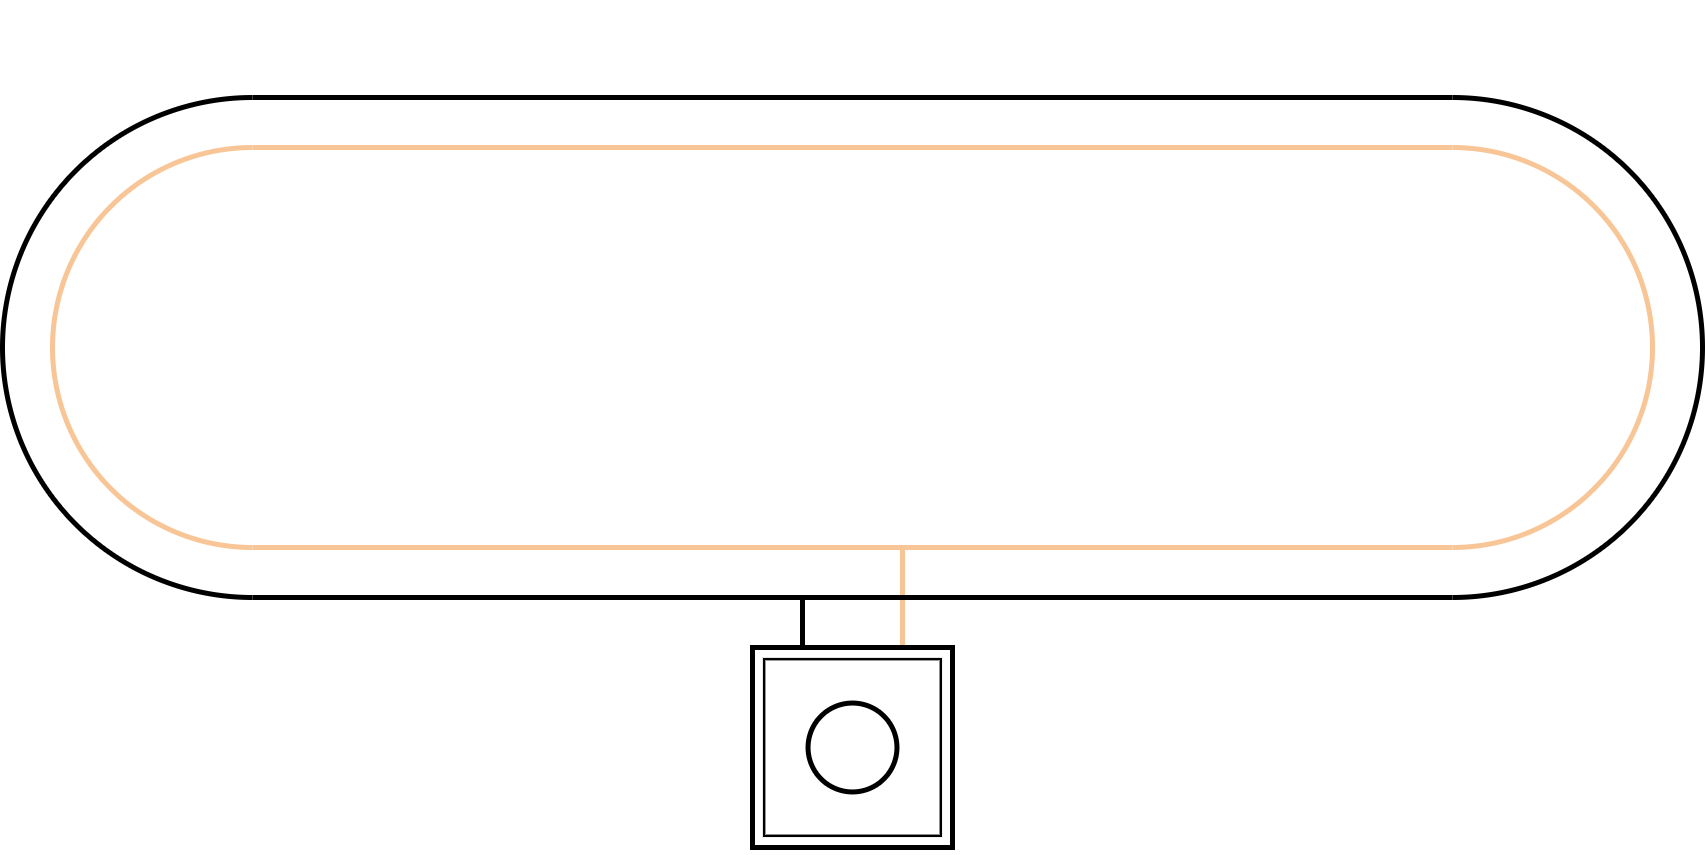
\includegraphics[width=\textwidth]{Assets/Images/2-Grundlagen/Modelleisenbahnen-Einfaches-Gleisoval.png}
    \caption{Einfaches Gleisoval mit regelbarem Trafo~\cite[nach][S. 180]{bib:Modellbauhandbuch}}\label{abb:Grundlagen:Steuerung-von-Modelleisenbahnen:Analoge-Steuerung:Einfaches-Gleisoval}
\end{figure}

Werden nun mehr als ein Zug auf das Gleisoval gesetzt, hat dies zur Folge, dass alle Züge gleichzeitig fahren. Sollen Züge unabhängig voneinander gesteuert werden, so muss das Gleisoval in mehrere Abschnitte unterteilt werden. Dafür werden die Gleise galvanisch getrennt und an die Abschnitte jeweils ein eigener Trafo angeschlossen.~\cite[][S. 181]{bib:Modellbauhandbuch} Bei anspruchsvolleren Anlagen, ist zusätzlich die Nutzung von Polwendeschaltern notwendig, um beispielsweise Gleisschleifen oder Gleisdreiecke zu ermöglichen.~\cite[][S. 183 f.]{bib:Modellbauhandbuch} Eine weitere Möglichkeit ist der Einbau von Schaltern, um bestimmte Gleisabschnitte vom Strom zu trennen.~\cite[][S. 182]{bib:Modellbauhandbuch}

Weichen werden auf einer analogen Modelleisenbahn wahlweise elektrisch oder manuell gestellt. Hierbei ist es der Kreativität des Modellbauers überlassen, wie er die Ansteuerung konkret umsetzt. Der Bau von Schaltbrettern, auf denen alle Weichen kompakt zusammengefasst sind, ist üblich.~\cite[][S. 185]{bib:Modellbauhandbuch} Dasselbe gilt für Signale, sofern man sich auf einer analogen Anlage für deren Einbau entscheidet.
\subsection{Digitale Steuerung}\label{text:Grundlagen:Steuerung-von-Modelleisenbahnen:Digitale-Steuerung}

Eine digitale Modelleisenbahn verfolgt ein grundlegend anderes Konzept. An den Gleisen liegt die ganze Zeit über eine konstante Spannung an. Die Lokomotiven leiten den Strom nicht mehr direkt an den Motor weiter, sondern sind mit einem Decoder ausgestattet. Dieser Decoder ist in der Lage, digitale Signale zu empfangen und in Steuerbefehle umzusetzen. Die Steuerbefehle werden über die Schienen an die Lokomotiven gesendet.

Die digitale Steuerung bietet gegenüber der analogen Steuerung einige Vorteile. So können mehrere Züge unabhängig voneinander gesteuert werden, ohne dass das Gleis in galvanisch getrennte Abschnitte unterteilt werden muss. Optional können Weichen und Signale ebenfalls digital gesteuert werden.

Durch den Einsatz digital gesteuerter Züge und Weichen ist eine Steuerung durch einen Computer möglich. Die gängigen Programme erlauben es, den Gleisplan schematisch nachzubauen und die gesamte Anlage per Mausklick zu steuern. Eine Vollautomatisierung der Anlage, wie es beispielsweise bei großen Anlagen zwingend notwendig ist, kann ebenfalls realisiert werden.

Für einen automatischen Betrieb der Anlage ist auch bei einer Modelleisenbahn eine Gleisfreimeldeanlage notwendig. Man spricht hier in der Regel von Rückmeldern. Realisiert werden sie über die Unterteilung der Strecke in Einspeiseabschnitte, die mit einem Rückmeldemodul verbunden sind. Fährt ein Zug in einen neuen Abschnitt ein, wird der Strom aus diesem Abschnitt gezogen und die neue Position ist somit bekannt. Hierfür ist eine präzise Konfiguration notwendig, da die Länge eines Zuges bekannt sein muss. Die exakte Position kann dann abgeschätzt werden.
